\chapter*{Introduction}
\label{introduction}
%
The goal of this paper is to analyse results from a study called \textit{Men and Bread} using Principal Component Analysis (PCA). \blankline
% 
<<<<<<< HEAD
In the study \textit{Men and Bread}, 21 subjects were asked to rate different types of buns according to different attributes. Nine different types of buns were presented, where one was presented as a familiarization with the scales. The buns presented in the study are shown in \autoref{fig:bread}, where bread B9 is the bun used for familiarization. 
=======
In the study \textit{Men and Bread} 21 subjects were asked to rate nine different types of buns according to different attributes. Nine different types of buns were presented where one was presented as a familiarization with the scales. The buns presented in the study are shown on \autoref{fig:bread}, where bread B9 is the bun used for familiarization. 
>>>>>>> ad024fa761c2fdb0b59931c6f6a1eb4b88ee637a
%
\begin{figure}[H]
\centering
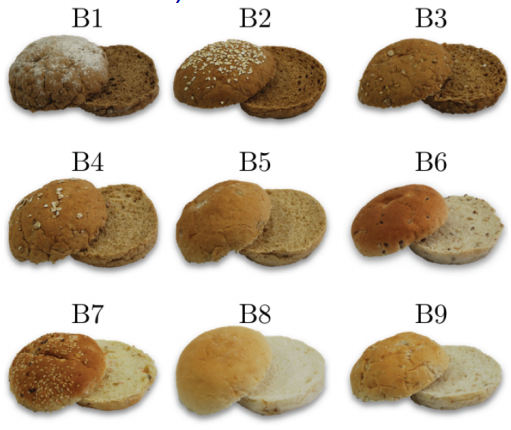
\includegraphics[width =0.7\textwidth]{Figure/Bread}
\caption{The different types of buns with identifying name, presented so that both crust and crumb can be seen.}
\label{fig:bread}
\end{figure}
\noindent
%
For each one of the different types of buns, 11 different attributes grouped in three different categories were rated. The attributes with the belonging scale question for each category are presented in \autoref{tab:DirectPerception}, \autoref{tab:AbstractPerception}, and \autoref{tab:Reflection}.
%
\begin{table}[H]
	\centering 
	\begin{tabular}{ |l|l| }
	\hline
	\multicolumn{2}{ |c| }{\textbf{Direct perception}} \\
	\hline
	\textit{Attribute} & \textit{Scale Question} \\ 
	\hline
	\multirow{2}{*}{Crust} & Hvilken farve har skorpen? (lys til mørk) \\
 	&  What color is the crust? (light to dark) \\ \hline
	\multirow{2}{*}{Crumb} &  Hvilken farve har krummen? (lys til mørk) \\
 	&  What color is the crumb? (light to dark) \\ \hline
	\multirow{2}{*}{Surface} & Hvilken tekstur har overfladen? (glat til ujævn) \\
 	&  What texture does the surface have? (smooth to uneven) \\ \hline
	\multirow{2}{*}{Seeds} & Hvor stor er andelen af kerner? (lav til høj) \\ 
 	&  How great is the amount of seeds? (small to large)\\ 
	\hline
	\end{tabular}
	\caption{Scale questions under the category: Direct perception. This category of questions are related to the readily available aspects of the bread.}
	\label{tab:DirectPerception}       
\end{table}
\noindent
%
\begin{table}[H]
	\centering 
	\begin{tabular}{ |l|l| }
	\hline
	\multicolumn{2}{ |c| }{\textbf{Abstract perception}} \\
	\hline
	\textit{Attribute} & \textit{Scale Question} \\ 
	\hline
	\multirow{2}{*}{Weight} &  Hvor tungt er brødet? (let til tungt) \\
 	&  How weighty is the bread? (light to heavy) \\ \hline
	\multirow{2}{*}{Density} & Hvor tæt er brødet? (luftigt til kompakt) \\
 	&  How dense is the bread? (airy to dense) \\ \hline
	\multirow{2}{*}{Juicy} &  Hvor saftigt er brødet? (tørt til svampet) \\
 	&  How juicy is the bread? (dry to moist) \\ 
 	\hline
	\end{tabular}
	\caption{Scale questions under the category: Abstract perception. This category relates to slightly more abstract concepts where the visual sense might not be the best tool for investigation.}
	\label{tab:AbstractPerception}       
\end{table}
\noindent
%
\begin{table}[H]
	\centering 
	\begin{tabular}{ |l|l| }
	\hline
	\multicolumn{2}{ |c| }{\textbf{Reflection}} \\
	\hline
	\textit{Attribute} & \textit{Scale Question} \\ 
	\hline
	\multirow{2}{*}{Filling} & Hvor mættende ser brødet ud? (lidt til meget) \\
 	&  How filling is the bread? (a little to a lot) \\ \hline
	\multirow{2}{*}{Nourishing} & Hvor nærende ser brødet ud? (usundt til sundt) \\
 	&   How nourishing is the bread? (healthy to unhealthy) \\ \hline
	\multirow{2}{*}{Wholegrain} & Hvor fuldkornsholdigt er brødet? (lidt til meget) \\
 	&   How large is the amount of wholegrain in the bread? (low to high) \\ \hline
	\multirow{2}{*}{Fibre} & Hvor fiberholdigt er brødet? (lidt til meget) \\ 
 	&   How fibrous is the bread? (low to high))\\ 
	\hline
	\end{tabular}
	\caption{Scale questions under the category: Reflection. This category concerns the qualities associated with bread. Qualities which are assumed to require a level of reflection.}
	\label{tab:Reflection}       
\end{table}
\noindent
%
Each scale question were presented to the test subjects with a scale. The scale used to rate the buns was a \textit{Visual Analogue Scale} (VAS) with open endpoints and an anchor point in the middle. An example of the scale used in the study is shown on \autoref{fig:Skala}. 
%
\begin{figure}[H]
\centering
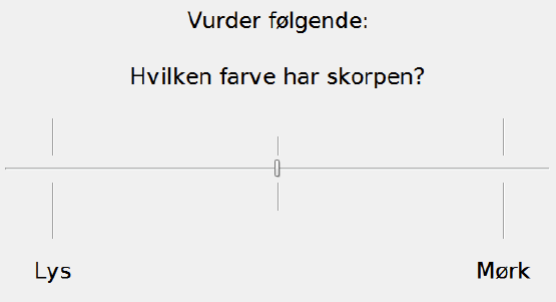
\includegraphics[width =0.7\textwidth]{Figure/Skala}
\caption{Example of the VAS used in the study \textit{Men and Bread}.}
\label{fig:Skala}
\end{figure}
\noindent


%Analyze the results from the example using PCA.

%First plot a “profile” of all stimuli.

%How much of the variance is explained by each component?

%(Plot a scree-plot including cumulative variance).

%Plot your PCA solution graphically. Both a plot with just your stimuli (scores) and a biplot with both scores and loadings.

%Make a table of the loadings of each word-pair on each principal component.

%Interpret the solution. Also, are there word-pairs that seem ”redundant” e.g. measures that same perceptual attribute?
